\begin{frame}
\frametitle{How to build the tree structure?}

\textbf{Goal}: Minimize $\lF{U}$/$\lF{V}$

\vspace{0.1in}
\parbox{10in}{
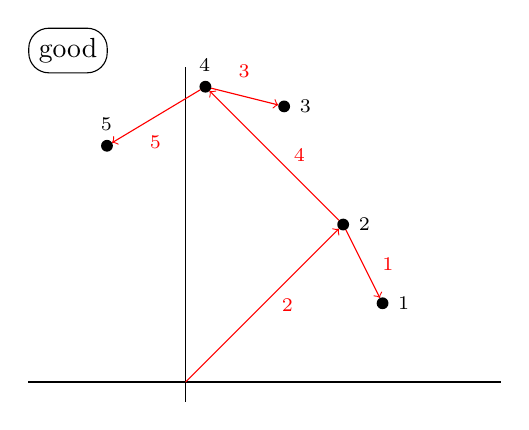
\begin{tikzpicture}
    [
    dot/.style = {minimum width=0.15cm,inner sep=0pt,line width=0pt,fill,circle,black,font=\small}
    ]
\draw[] (0,4) -- (0,-0.25);
\draw[] (4,0) -- (-2,0);
\node[dot,label={0:$\w_1$}] (w1) at (2.5,1) {};
\node[dot,label={0:$\w_2$}] (w2) at (2,2) {};
\node[dot,label={90:$\w_4$}] (w4) at (0.25,3.75) {};
\node[dot,label={0:$\w_3$}] (w3) at (1.25,3.5) {};
\node[dot,label={$\w_5$}] (w5) at (-1,3) {};

\draw[->,color=red] (0,0) -- node[label={0:$\uu_2$}]{} (w2);
\draw[->,color=red] (w2) -- node[label={0:$\uu_1$}]{} (w1);
\draw[->,color=red] (w2) -- node[label={0:$\uu_4$}]{} (w4);
\draw[->,color=red] (w4) -- node[label={$\uu_3$}]{} (w3);
\draw[->,color=red] (w4) -- node[label={270:$\uu_5$}]{} (w5);

\node[anchor=north west, draw, rounded corners=0.1in, inner sep=0.05in] at (-2,4.5) {good};
\end{tikzpicture}
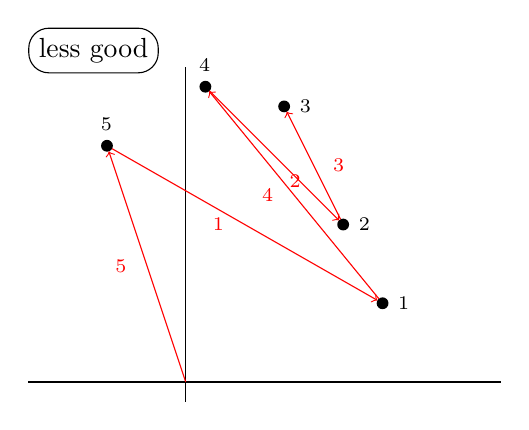
\begin{tikzpicture}
    [
    dot/.style = {minimum width=0.15cm,inner sep=0pt,line width=0pt,fill,circle,black,font=\small}
    ]
\node[anchor=north west, draw, rounded corners=0.1in, inner sep=0.05in] at (-2,4.5) {less good};
\draw[] (0,4) -- (0,-0.25);
\draw[] (4,0) -- (-2,0);
\node[dot,label={0:$\w_1$}] (w1) at (2.5,1) {};
\node[dot,label={0:$\w_2$}] (w2) at (2,2) {};
\node[dot,label={90:$\w_4$}] (w4) at (0.25,3.75) {};
\node[dot,label={0:$\w_3$}] (w3) at (1.25,3.5) {};
\node[dot,label={$\w_5$}] (w5) at (-1,3) {};

\draw[->,color=red] (0,0) -- node[label={180:$\uu_5$}]{} (w5);
\draw[->,color=red] (w5) -- node[label={180:$\uu_1$}]{} (w1);
\draw[->,color=red] (w1) -- node[label={180:$\uu_4$}]{} (w4);
\draw[->,color=red] (w4) -- node[label={300:$\uu_2$}]{} (w2);
\draw[->,color=red] (w2) -- node[label={0:$\uu_3$}]{} (w3);
\end{tikzpicture}
}
%\vspace{0.1in}

%\vspace{0.1in}
\pause
\begin{block}{Lemma 2 (informal)}
For all $U$/$V$-tree structures,
%\begin{equation}
$\lF{V} \le \lF{U} \le 2\lF{W} \le 2\sqrt{kd}.$
%\end{equation}
\end{block}

\textbf{Intuition:} There's no ``bad'' way to make a tree.

\end{frame}

